\documentclass[aspectratio=169,11pt]{beamer}
\usetheme{default}
\usefonttheme{serif}
\setbeamertemplate{navigation symbols}{}
\setbeamertemplate{itemize items}[circle]

\usepackage{tikz}
\usetikzlibrary{arrows.meta,positioning,calc}
\usepackage{pgfplots}
\pgfplotsset{compat=1.18}
\usepackage{booktabs}
\usepackage{xcolor}
\usepackage{array}

\definecolor{ink}{HTML}{1F2328}
\definecolor{muted}{HTML}{6A737D}
\definecolor{faint}{HTML}{EEF0F3}
\definecolor{accent}{HTML}{1F6FEB}
\definecolor{good}{HTML}{1A7F37}
\definecolor{bad}{HTML}{CF222E}
\definecolor{warn}{HTML}{BF8700}
\definecolor{g1}{HTML}{C9D1D9}
\definecolor{g2}{HTML}{8C959F}
\definecolor{g3}{HTML}{57606A}

\setbeamercolor{normal text}{fg=ink}
\setbeamercolor{frametitle}{fg=ink}
\setbeamercolor{title}{fg=ink}
\setbeamercolor{structure}{fg=accent}
\setbeamercolor{block title}{bg=faint,fg=ink}
\setbeamercolor{block body}{bg=faint!50,fg=ink}
\setbeamercolor{block title alerted}{bg=bad!12,fg=ink}
\setbeamercolor{block body alerted}{bg=bad!6,fg=ink}
\setbeamercolor{block title example}{bg=good!12,fg=ink}
\setbeamercolor{block body example}{bg=good!6,fg=ink}
\setbeamerfont{frametitle}{size=\Large,series=\bfseries}

\setbeamertemplate{frametitle}{%
  \vspace{0.45em}\insertframetitle\par\vspace{-0.15em}%
  {\color{g1}\rule{\textwidth}{0.4pt}}}
\setbeamertemplate{footline}{%
  \hfill{\color{muted}\scriptsize\insertframenumber\,/\,\inserttotalframenumber}\hspace{1.2em}\vspace{0.6em}}

\newcommand{\src}[1]{\par\vfill\begin{minipage}{0.96\textwidth}\color{muted}\tiny #1\end{minipage}\vspace{-0.2em}}
\newcommand{\bignum}[3][ink]{%
  \begin{tabular}{@{}c@{}}
    {\color{#1}\fontsize{18}{20}\selectfont\bfseries #2}\\[3pt]
    \parbox{3.2cm}{\centering\scriptsize\color{muted} #3}
  \end{tabular}}
\pgfplotsset{
  deck/.style={
    ybar, bar shift=0pt, axis lines*=left, ymajorgrids, grid style={faint},
    tick label style={font=\footnotesize, color=ink},
    label style={font=\footnotesize, color=ink},
    xticklabel style={align=center, font=\footnotesize},
    every node near coord/.append style={font=\scriptsize, color=ink,
      /pgf/number format/fixed, /pgf/number format/precision=1},
    nodes near coords, clip=false,
    enlarge x limits=0.35,
  },
}

\newcommand{\Fresh}{Fresh set: 200 MATH questions the practice comparison never saw. Depth 3, 32 slots, one seed, one run per arm.}
\newcommand{\Pins}{Ouro-1.4B, stock prompt, temperature 0.6, top-$p$ 0.95, math-verify 0.9.0. Four samples; the most common boxed answer is kept.}

\title{Forcing a short answer looked like a 6-point win}
\subtitle{On fresh questions it was +1.5, and that is chance}
\date{November 2026}

\begin{document}

%-------------------------------------------------------------
\begin{frame}[plain]
  \vspace{0.7em}
  {\color{muted}\small Looped serving \;$\cdot$\; Ouro-1.4B \;$\cdot$\; MATH}\\[0.55em]
  {\Large\bfseries Forcing a short answer looked like a 6-point win.}\\[0.15em]
  {\Large\bfseries On fresh questions it was +1.5, and that is chance.}\\[0.65em]
  {\color{muted}\small The model writes either a long monologue or a short worked solution.
  On 400 practice questions the short form won. A fresh 200 did not repeat that.
  What did repeat is the length limit on the monologue.}
  \vspace{0.85em}
  \begin{center}
  \begin{tabular}{@{}c@{\hspace{0.9em}}c@{\hspace{0.9em}}c@{}}
    \bignum{+1.5 pts}{Fresh set. Direct minus natural, cap 2{,}048.} &
    \bignum[good]{+6.0 pts}{Fresh set. Same monologue, cap raised to 4{,}096.} &
    \bignum{26 s vs.\ 92 s}{Mean time. Direct answer versus the longer monologue.} \\
  \end{tabular}
  \end{center}
  \vspace{0.75em}
  \begin{exampleblock}{What this talk can say}
    On this workload a direct answer is the faster operating point, and letting the natural
    monologue run to 4{,}096 tokens is what raises held-out accuracy.
  \end{exampleblock}
\end{frame}

%-------------------------------------------------------------
\begin{frame}{Two ways an answer can start}
  Ouro repeats the same layers on every word. These runs repeat them three times.
  What we change is the first word of the answer.
  \vspace{0.7em}
  \begin{columns}[c]
    \begin{column}{0.55\textwidth}
      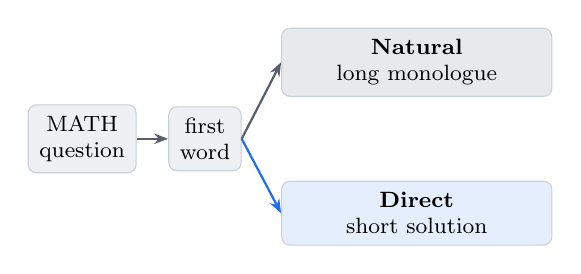
\begin{tikzpicture}[
          box/.style={draw=g1, fill=faint, rounded corners=3pt, align=center,
                      font=\footnotesize, inner sep=4pt},
          arr/.style={-{Stealth[length=5pt]}, thick, g3}]
        \node[box] (q) {MATH\\question};
        \node[box, right=0.4cm of q] (first) {first\\word};
        \node[box, fill=g3!14, text width=3.15cm, above right=0.12cm and 0.5cm of first] (think)
          {\textbf{Natural}\\long monologue};
        \node[box, fill=accent!12, text width=3.15cm, below right=0.12cm and 0.5cm of first] (to)
          {\textbf{Direct}\\short solution};
        \draw[arr] (q) -- (first);
        \draw[arr] (first.east) -- (think.west);
        \draw[arr, accent] (first.east) -- (to.west);
      \end{tikzpicture}
    \end{column}
    \begin{column}{0.42\textwidth}
      {\small Direct does not turn reasoning off. It starts the answer with the word ``To'', which this model uses for a short solution.}
      \vspace{0.7em}

      {\small Natural lets the model choose. On these questions that choice often opens a monologue, and the monologue runs into the length cap.}
    \end{column}
  \end{columns}
  \src{Each question is asked four times. The boxed answer that appears most often is the one we grade.}
\end{frame}

%-------------------------------------------------------------
\begin{frame}{Practice set, then a fresh check}
  The practice set formed the idea. The fresh set is the same comparison on questions that idea never saw.
  \begin{columns}[T]
    \begin{column}{0.48\textwidth}
      \begin{block}{Practice set \textnormal{\small\textcolor{muted}{--- form the idea}}}
        \small
        \begin{itemize}\setlength\itemsep{0.08em}
          \item 400 MATH questions, balanced by difficulty
          \item Depth-3 engine, cap 2{,}048
          \item This is the +6.25 point result
        \end{itemize}
        \vspace{0.05em}
        {\scriptsize\color{muted} A longer cap, depth 2, depth 4, and a monologue
        fallback were checked here later, for accuracy. Their times are left out.}
      \end{block}
    \end{column}
    \begin{column}{0.48\textwidth}
      \begin{block}{Fresh set \textnormal{\small\textcolor{muted}{--- check the idea}}}
        \small
        \begin{itemize}\setlength\itemsep{0.08em}
          \item 200 questions, held out from the practice set
          \item Depth 3, with 32 questions in flight at once
          \item One seed. One run of each arm, back to back
        \end{itemize}
        \vspace{0.05em}
        {\scriptsize\color{muted} The arms were not shuffled together, so a slow
        drift in the machine is not averaged out. Each time is a single run.}
      \end{block}
    \end{column}
  \end{columns}
  \src{\Pins}
\end{frame}

%-------------------------------------------------------------
\begin{frame}{The result that looked like a paper}
  On the 400 practice questions, forcing the short answer gained 6.25 points.
  The interval is +3.0 to +9.5. Thirty-six questions were right only in the short-answer
  run, against 11 the other way. Paired test, $p = 0.00035$.
  \vspace{0.15em}
  \begin{center}
  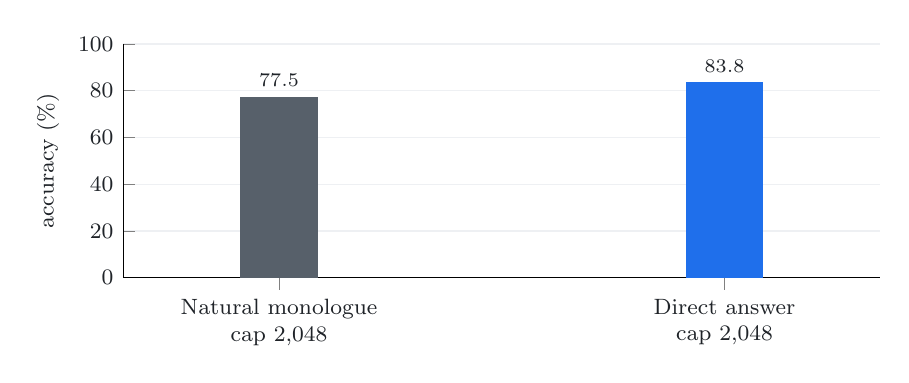
\begin{tikzpicture}
    \begin{axis}[deck, width=11.2cm, height=4.55cm, bar width=28pt,
        ymin=0, ymax=100, ylabel={accuracy (\%)},
        xtick={0,1},
        xticklabels={{Natural monologue\\cap 2{,}048},{Direct answer\\cap 2{,}048}}]
      \addplot[fill=g3, draw=none] coordinates {(0,77.5)};
      \addplot[fill=accent, draw=none] coordinates {(1,83.8)};
    \end{axis}
  \end{tikzpicture}
  \end{center}
  \src{Practice set, 400 questions. 95\% intervals 73.2--81.5 and 80.0--87.2.
  The gap sat on the 92 questions where every natural sample opened as a monologue: 32\% versus 61\%.
  29.9\% of monologue samples hit the 2{,}048 cap; 2.2\% of direct answers did.}
\end{frame}

%-------------------------------------------------------------
\begin{frame}{On fresh questions that gain is gone}
  Same comparison, 200 questions the practice set never saw.
  Direct is 79.5\% and the natural monologue is 78.0\%.
  \vspace{0.1em}
  \begin{columns}[c]
    \begin{column}{0.62\textwidth}
      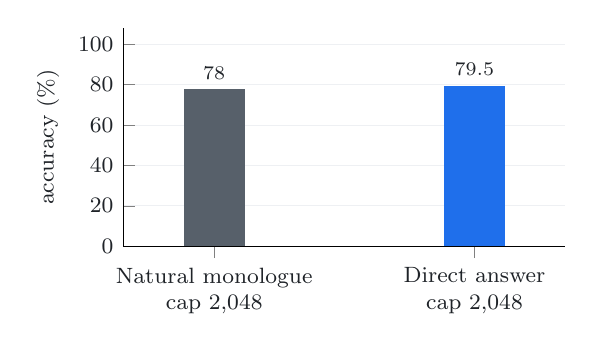
\begin{tikzpicture}
        \begin{axis}[deck, width=7.2cm, height=4.35cm, bar width=22pt,
            ymin=0, ymax=108, ylabel={accuracy (\%)},
            ytick={0,20,40,60,80,100},
            xtick={0,1},
            xticklabels={{Natural monologue\\cap 2{,}048},{Direct answer\\cap 2{,}048}}]
          \addplot[fill=g3, draw=none] coordinates {(0,78.0)};
          \addplot[fill=accent, draw=none] coordinates {(1,79.5)};
        \end{axis}
      \end{tikzpicture}
    \end{column}
    \begin{column}{0.36\textwidth}
      \bignum{+1.5}{direct minus natural, points}\\[0.7em]
      \bignum[warn]{$p = 0.581$}{interval $-2.0$ to $+5.0$}\\[0.55em]
      {\scriptsize\color{muted} Eight questions only the direct run got right, five the other way.
      That accuracy gain is withdrawn. The longer cap is the next slide.}
    \end{column}
  \end{columns}
  \src{\Fresh\ 95\% intervals 72.0--83.5 and 74.0--85.0. Paired bootstrap, 10{,}000 draws, seed 0.}
\end{frame}

%-------------------------------------------------------------
\begin{frame}{What did repeat is the length limit}
  At 2{,}048 tokens, 27\% of fresh monologue samples hit the cap.
  Raising it to 4{,}096 cuts that to 18\% and lifts accuracy by 6 points
  (interval +2 to +10, 15 questions gained and 3 lost, $p = 0.0075$).
  \vspace{0.2em}
  {\scriptsize
  \renewcommand{\arraystretch}{1.12}
  \begin{tabular}{@{}l l r r r@{}}
    \toprule
    \textbf{Comparison} & \textbf{Set} & \textbf{Difference} & \textbf{Interval} & \textbf{$p$} \\
    \midrule
    Monologue 4{,}096 vs.\ 2{,}048 & Fresh, 200 & +6.0 pts & +2.0 to +10.0 & 0.0075 \\
    Monologue 4{,}096 vs.\ direct & Fresh, 200 & +4.5 pts & +1.0 to +8.0 & 0.022 \\
    \addlinespace
    Monologue 4{,}096 vs.\ 2{,}048 & Practice, 400 & +5.0 pts & +2.0 to +8.2 & 0.0029 \\
    Monologue 4{,}096 vs.\ direct & Practice, 400 & $-1.25$ pts & $-4.5$ to +2.0 & 0.53 \\
    \bottomrule
  \end{tabular}}
  \vspace{0.25em}
  \begin{block}{Reading}
    \small The practice-set win was the 2{,}048 cap cutting monologues off before they boxed an answer.
    Once a monologue can finish, it ties the short answer on the practice set and leads it on the fresh set.
  \end{block}
  \src{Paired by question. The 4{,}096 monologue charges about 19{,}700 loop-tokens a question; the direct answer, about 9{,}200.}
\end{frame}

%-------------------------------------------------------------
\begin{frame}{The short answer is the fast one}
  On the fresh set every arm shared one depth-3 engine and 32 slots.
  The direct answers finish. The longer monologue is the accurate arm and the slow one.
  \vspace{0.05em}
  \begin{columns}[c]
    \begin{column}{0.60\textwidth}
      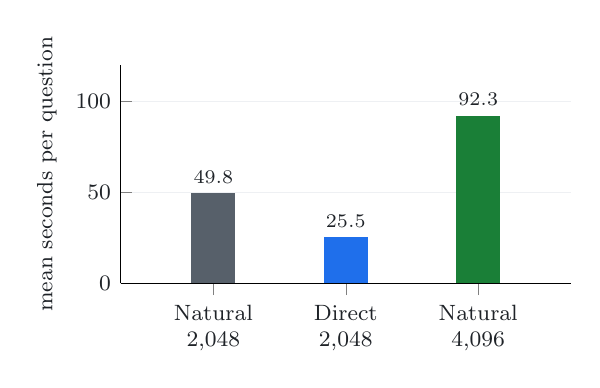
\begin{tikzpicture}
        \begin{axis}[deck, width=7.3cm, height=4.35cm, bar width=16pt,
            ymin=0, ymax=120, ylabel={mean seconds per question},
            xtick={0,1,2},
            xticklabels={{Natural\\2{,}048},{Direct\\2{,}048},{Natural\\4{,}096}}]
          \addplot[fill=g3, draw=none] coordinates {(0,49.8)};
          \addplot[fill=accent, draw=none] coordinates {(1,25.5)};
          \addplot[fill=good, draw=none] coordinates {(2,92.3)};
        \end{axis}
      \end{tikzpicture}
    \end{column}
    \begin{column}{0.38\textwidth}
      \bignum[accent]{20.4 / min}{direct, cap 2{,}048}\\[0.7em]
      \bignum{11.5 / min}{natural, cap 2{,}048}\\[0.7em]
      \bignum{6.5 / min}{natural, cap 4{,}096}\\
    \end{column}
  \end{columns}
  \src{\Fresh\ 95th percentile: 82\,s, 65\,s, and 209\,s. One run each, back to back.
  Cutting generated work on a token-clock replay is not a live latency result.}
\end{frame}

%-------------------------------------------------------------
\begin{frame}{Depth and a fallback, on the practice set}
  These checks close the practice-set idea. They are not a fresh-set result.
  With the answer forced short, depth 4 matches depth 3 exactly, and depth 2 loses 8.75 points.
  \vspace{0.05em}
  \begin{columns}[c]
    \begin{column}{0.50\textwidth}
      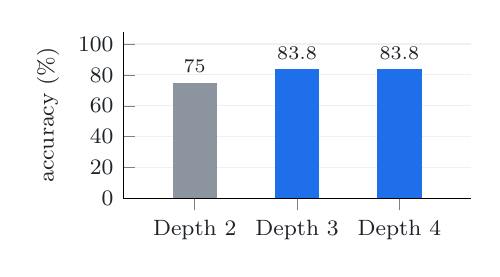
\begin{tikzpicture}
        \begin{axis}[deck, width=6.0cm, height=3.7cm, bar width=16pt,
            ymin=0, ymax=108, ylabel={accuracy (\%)},
            ytick={0,20,40,60,80,100},
            xtick={0,1,2},
            xticklabels={{Depth 2},{Depth 3},{Depth 4}}]
          \addplot[fill=g2, draw=none] coordinates {(0,75.0)};
          \addplot[fill=accent, draw=none] coordinates {(1,83.8)};
          \addplot[fill=accent, draw=none] coordinates {(2,83.8)};
        \end{axis}
      \end{tikzpicture}
    \end{column}
    \begin{column}{0.48\textwidth}
      \begin{block}{Think fallback, 75 questions}
        \small The practice questions where four direct answers never reached a 3-of-4 agreement.
        Two monologue samples, cap 4{,}096, scored \textbf{28\%}.
        Direct on those same 75 scored 30.7\%.
        \vspace{0.25em}

        {\scriptsize\color{muted} 83\% of those samples hit the cap. Mean wait 199\,s.
        This 28\% is not a score on all 400.}
      \end{block}
    \end{column}
  \end{columns}
  \src{Practice set, direct answers, cap 2{,}048.
  Depth 4 ties depth 3 (15 questions each way, $p = 1$) and uses 12{,}059 loop-tokens per question against 9{,}118.
  Depth 2: $-12.2$ to $-5.2$, 9 against 44, $p = 1.2\times 10^{-6}$.}
\end{frame}

%-------------------------------------------------------------
\begin{frame}{What this talk can say}
  \scriptsize
  \begin{itemize}\setlength\itemsep{0.7em}
    \item \textcolor{bad}{\textbf{Withdrawn.}}
          +6.25 points on 400 practice questions; +1.5 on 200 fresh questions, $p = 0.581$.
    \item \textcolor{good}{\textbf{Holds, both sets.}}
          Cap 4{,}096 versus 2{,}048 is +6.0 on the fresh set and +5.0 on the practice set.
    \item \textcolor{accent}{\textbf{Holds, fresh set.}}
          Same cap: short answer 25.5\,s, monologue 49.8\,s. One run of each arm.
    \item \textbf{No.}
          Depth 4 ties depth 3 at 83.8\% on the practice set. Depth 2 is 75.0\%.
    \item \textbf{No.}
          On 75 unsettled practice questions the monologue scores 28\%; the direct vote scores 30.7\%.
  \end{itemize}
  \vspace{0.35em}
  \begin{exampleblock}{The operating point}
    \small On this Ouro-1.4B workload, a direct answer is the faster operating point, and letting
    the natural monologue run to 4{,}096 tokens is what raises held-out accuracy.
    Cutting generated work did not by itself make the model faster in a way you can claim from the token-clock replay.
  \end{exampleblock}
\end{frame}

\end{document}
